%!TEX root = thesis.tex


\chapter{Content-Aware Collaborative Music Recommendation}\label{chpt:content}


Although content is fundamental to our music listening preferences (or at least we believe so), the leading performance in music recommendation is achieved by collaborative filtering methods which exploit the similarity patterns in user's listening history rather than the audio content of songs. Meanwhile, collaborative filtering has the well-known ``cold-start'' problem, i.e., it is unable to work with new songs that no one has listened to.  Efforts on incorporating content information into collaborative filtering methods have shown success in many non-musical applications, such as scientific article recommendation. Inspired by the related work, we train a neural network on semantic tagging information as a content model and use it as a prior in a collaborative filtering model. Such a system still allows the user listening data to ``speak for itself''. The proposed system is evaluated on the Million Song Dataset and shows comparably better result than the collaborative filtering approaches, in addition to the favorable performance in the cold-start case. 

%
\section{Introduction}\label{chpt:content:sec:intro}
Music recommendation is an important yet difficult task in \gls{MIR}. A recommendation system that accurately predicts users' listening preferences bares enormous commercial value. However, the high complexity and dimensionality of music data and the scarcity of user feedback makes it difficulty to create a successful music recommendation system. 

Two primary approaches exist in recommendation\footnote{Collective intelligence also plays a huge role in commercial recommender systems. However, it is beyond the scope of this dissertation.}: collaborative filtering and content-based methods. For music, the state-of-the-art recommendation results have been achieved by collaborative filtering methods (e.g., all the top-ranked submissions to the Kaggle Million Song Dataset Challenge\footnote{\url{https://www.kaggle.com/c/msdchallenge}} are based on collaborative filtering even though the dataset also comes with content features and meta-data), which requires only information on users' listening history rather than the musical content for recommendation. The central assumption of this model is that a user is likely to accept a song that is liked by users who have similar taste.  A major category of collaborative filtering approaches is based on latent factor (matrix factorization) model. It assumes that a low-dimensional representation exists for both users and songs such that the compatibility between a user and a song, modeled as their inner product in this latent space, predicts the user's fondness of the song. As discussed in \Cref{chpt:background:sec:data}, in the case that user feedback is \emph{implicit} (e.g., whether or not the user has listened to a particular song), \gls{WMF} \citep{hu2008collaborative} works particularly well. \gls{WMF} is described in \Cref{chpt:background:sec:cf_implicit}.

On the other hand, modeling musical content for the purpose of taste prediction is difficult due to the structural complexity present in music data which is hard to capture by simple models. Deep learning has shown its power in various pattern recognition tasks with its capability of extracting hierarchical representations from raw data. In music recommendation, \citet{van2013deep} have experimented with neural networks on predicting the song latent representation from musical content.  

It is natural to combine collaborative filtering and content models in recommendation to utilize different sources of information. A successful attempt from \citet{wang2011collaborative}, which joins a content model on article with collaborative filtering, achieves good performance on scientific article recommendation.

Inspired by these mentioned above, we create a content-aware collaborative music recommendation system. As the name suggests, the system has two components: the content model and the collaborative filtering model. To obtain a powerful content model, we pre-train a multi-layer neural network to predict semantic tags from vector-quantized acoustic feature. The output of the last hidden layer is treated as a high-level representation of the musical content, which is used as a prior for the song latent representation in collaborative filtering. We evaluate our system on the Million Song Dataset and show competitive performance to the state-of-the-art system.



\section{Related work}\label{chpt:content:sec:related}

In this section we review two closely relevant models: collaborative topic model for article recommendation and deep content-based music recommendation. We also review other related work which hybridizes content and collaborative filtering models.  

% \subsection{Recommendation by matrix factorization}\label{sec:huetal}

% In a matrix factorization recommendation model, we represent both users and items in a shared low-dimensional space of dimension $K$, where user $u$ is represented by a latent factor $\mb\theta_u \in \RR^K$ and item $i$ is represented by a latent factor $\mb\beta_i \in \mathbb{R}^K$. To make a prediction about the preference of user $u$ on item $i$, we simply take the dot product between the two $\hat{r}_{ui} = \mb\theta_u^\top \mb\beta_i$. To estimate user and item factors, we can minimize the squared loss between the estimated preference and actual responses $\sum_{u, i} (r_{ui} - \hat{r}_{ui})^2$,  with $\ell_2$ regularization on the factors to prevent overfitting. Alternating least squares (ALS) can be employed for efficient optimization. Equivalently, we can formulate a probabilistic matrix factorization model \cite{mnih2007probabilistic} with the following generative process:
% \begin{itemize}
% \item For each user $u$, draw user latent factor:
% \vspace{-0.05in}
% \[\mb\theta_u \sim \mathcal{N}(0, \lambda_\theta^{-1} I_K),\]
% \item \vspace{-0.08in}
% For each item $i$, draw item latent factor:
% \vspace{-0.05in}
% \[\mb\beta_i \sim \mathcal{N}(0, \lambda_\beta^{-1} I_K),\]
% \item \vspace{-0.08in}
% For each user-item pair $(u, i)$, draw feedback: 
% \[r_{ui} \sim \mathcal{N}(\mb\theta_u^\top\mb\beta_i, c_{ui}^{-1}),\]
% \end{itemize}
% \vspace{-0.08in}
% and obtain the same estimates via maximum \emph{a posteriori}. 
% Here $c_{ui}$ represents our confidence on the corresponding response $r_{ui}$, i.e., larger value of $c_{ui}$ indicates that there is less uncertainty about the response $r_{ui}$, and vice versa. 
% This is especially crucial in the case of implicit feedback (e.g., whether user $u$ listened to song $i$), because of its noisy nature. 
% Hu et al. \cite{hu2008collaborative} propose a simple heuristic for setting the values of $c_{ui}$ for implicit feedback \footnote{In \cite{hu2008collaborative}, the observational model is on the binary indicator variable $p_{ui}= \mathbb{I}\{r_{ui} > 0\}$ rather than $r_{ui}$, 
% i.e., $p_{ui} \sim \mathcal{N}(\mb\theta_u^\top\mb\beta_i, c_{ui}^{-1})$. 
% However, in this paper the response $r_{ui}$ is itself binary, indicating whether user $u$ has listened to song $i$.
% Thus we treat $r_{ui}$ and $p_{ui}$ interchangeably.
% }:
% \[c_{ui} = 1 +  \alpha \log(1 + r_{ui} / \epsilon)\]
% where $\alpha$ and $\epsilon$ are tunable hyperparameters. This method achieves the state-of-the-art recommendation performance in the implicit feedback case.

\subsection{Collaborative topic model}\label{chpt:content:sec:ctm}

As reviewed in \Cref{chpt:background:sec:cf}, a widely used approach to recommender systems is collaborative filtering, where items are recommended to a user based on other
users with similar patterns of item consumption. Matrix factorization models \citep{hu2008collaborative, koren2009matrix} are among the most successful collaborative filtering methods. In the case of the Gaussian matrix factorization \citep{salakhutdinov2007probabilistic}, efficient \textit{alternating least squares} update (\Cref{chpt:background:algo:gmf,chpt:background:algo:wmf}) exists for scalable inference, makes it an attractive option for commercial recommender systems.

Due to its content-free nature, collaborative filtering approaches can be applied in a wide range of domains. They perform well on what is called \emph{in-matrix} predictions, i.e., recommending items that have been consumed by some users. However, this approach suffers from the well-known problem that it is unable to recommend new items that no user has consumed, or making \emph{out-of-matrix} predictions, where content-based models are better suited. \Cref{chpt:content:fig:in_and_out} provides illustrative examples for both \emph{in-matrix} and \emph{out-of-matrix} predictions. Many efforts have been made to incorporate content into collaborative filtering. \citet{wang2011collaborative} propose the \gls{CTR} model for scientific article recommendation, which is particularly relevant to our proposed method.  

\begin{figure}
  \centering
    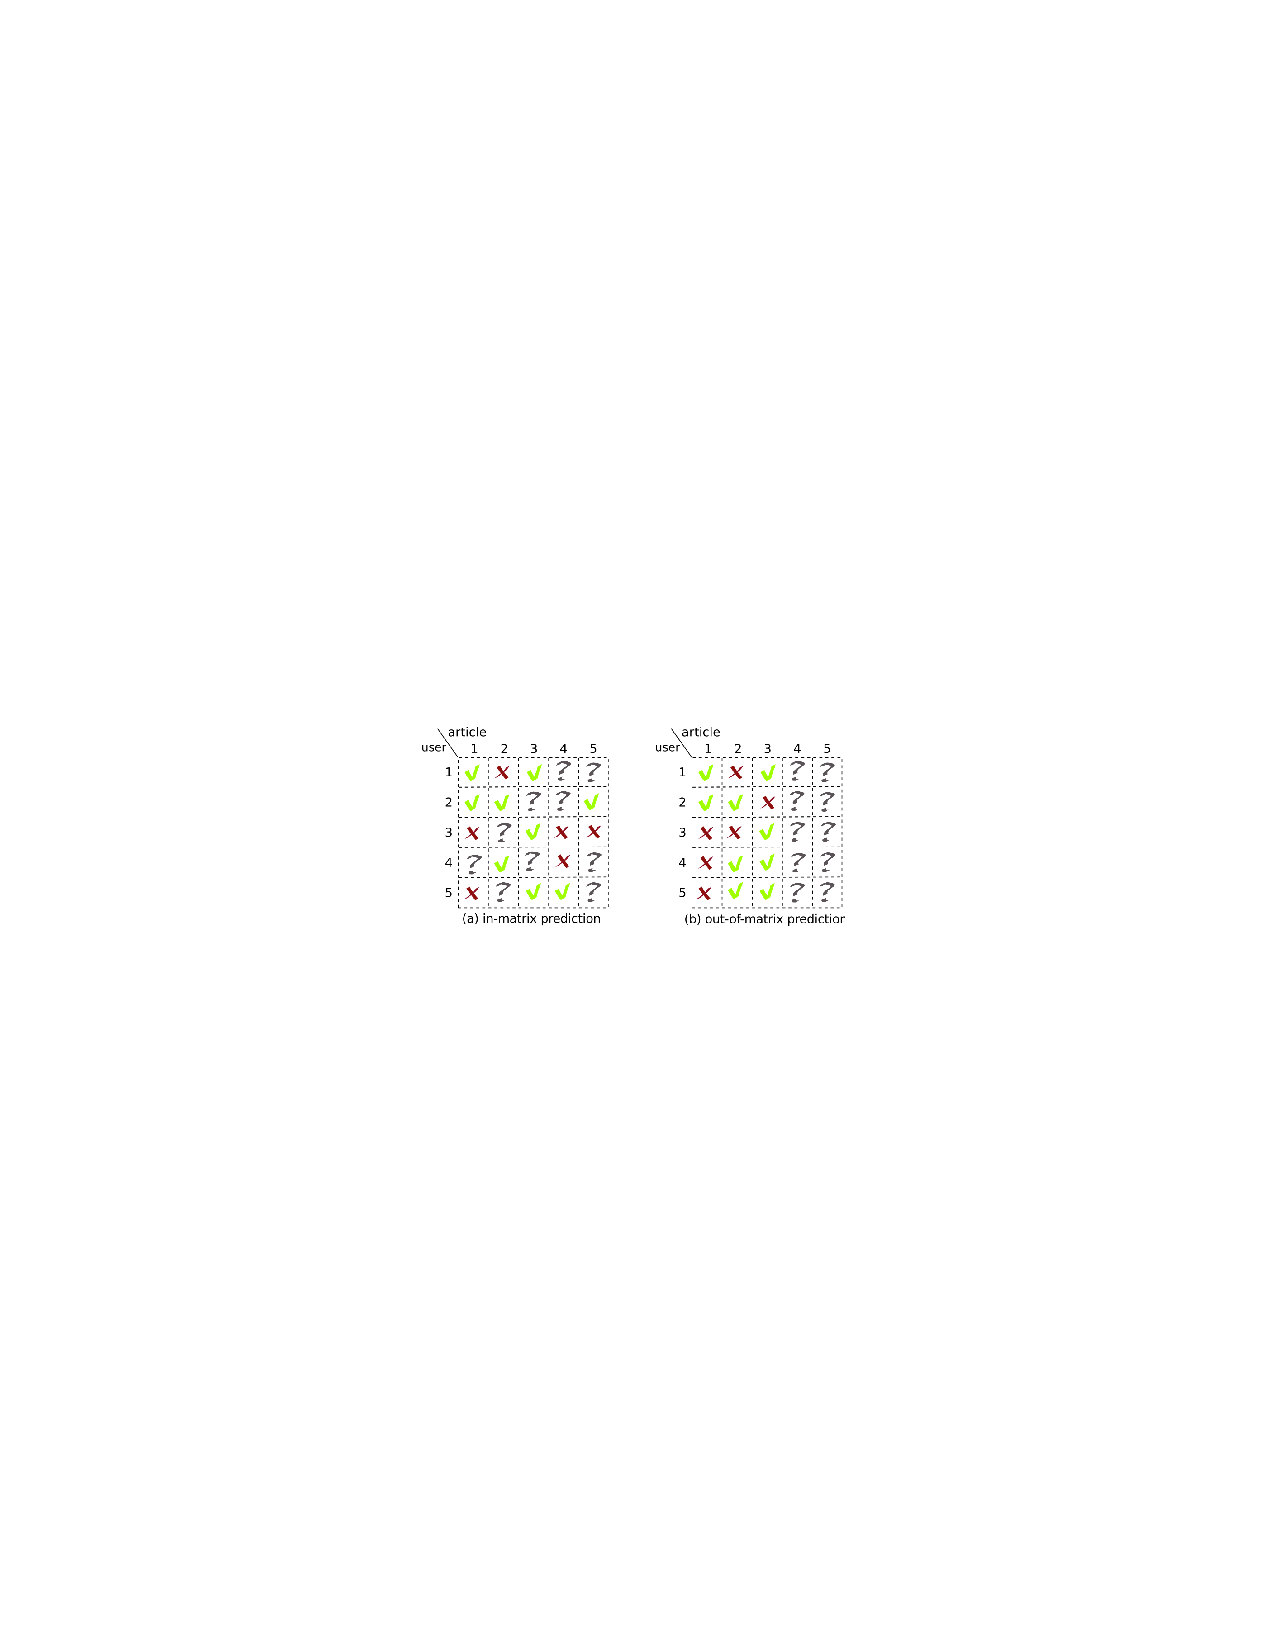
\includegraphics[width=\textwidth]{fig/in_and_out_matrix}
      \caption{An illustration of the \emph{in-matrix} (left) and \emph{out-of-matrix} (right) predictions, where $\checkmark$ indicates ``like'', $\mathrm{x}$ indicates ``dislike'', and $?$ indicates ``unknown''. Copied from \citet{wang2011collaborative}.}
      \label{chpt:content:fig:in_and_out}
\end{figure}

There are two components in \gls{CTR}: a matrix factorization collaborative filtering model (\gls{WMF} as described in \Cref{chpt:background:sec:cf_implicit}) and a \gls{LDA} article content model. \gls{LDA} \citep{blei2003latent} is a mixed-membership model on documents. Assuming there are $K$ topics $\Phi = \mb\phi_{1:K}$, each of which is a distribution over a fixed set of vocabulary, \gls{LDA} treats each document as a mixture of these topics where the topic proportion $\mb\pi_i$ is inferred from the data.
One can understand \gls{LDA} as representing documents in a low-dimensional ``topic'' space with the topic proportion being their coordinates. With this interpretation, the generative process of \gls{CTR} is as follows: 
\begin{itemize}
\item For user $u = 1, \dots, U$, draw user latent factor: $\mb\theta_u \sim \cN(\bzero, \lambda_\theta^{-1} \mathrm{I}_K)$,
\item For document $i = 1, \dots, I$, 
\begin{itemize}
\item Draw topic proportion $\mb\pi_i \sim \dir(\alpha)$,
\item For word $n$ in document $i$, 
\begin{itemize}
\item 
Draw topic assignment $z_{in} \sim \discrete(\mb\pi_i)$,
\item 
Draw word $w_{in} \sim \discrete(\mb\phi_{z_{in}})$,
\end{itemize}
\item Draw latent factor $\mb\beta_i \sim \cN(\mb\pi_i, \lambda_\beta^{-1} \mathrm{I}_K)$,
 \end{itemize}
\item For user-document pair $(u, i)$, draw feedback: $r_{ui} \sim \cN(\mb\theta_u^\top\mb\beta_i, c_{ui}^{-1})$.
\end{itemize}

Here the confidence $c_{ui}$ is set the same as in \gls{WMF}. We can see \gls{CTR} differs from \gls{WMF} in that \gls{CTR} assumes that the item latent factor $\mb\beta_i$ is close to the topic proportion $\mb\pi_i$ but could deviate from it if necessary. This allows the user-item interaction data to ``speak for itself''. An attractive characteristic of \gls{CTR} is its capability of making \emph{out-of-matrix} predictions.  This is done by using the topic proportion $\mb\pi_i$ alone as the item latent factor: $\hat{r}_{ui} = \mb\theta_u^\top \mb\pi_i$, which is not possible in the traditional collaborative filtering model. 

Although \gls{CTR} achieves better recommendation performance than \gls{WMF}, it does not scale well with large data. Since the model is not conditionally conjugate: the prior on $\mb\beta_i$ comes from a Dirichlet-distributed random variable $\mb\pi_i$, topic proportion $\mb\pi_i$ cannot be updated analytically and slower numerical optimization method is required. 
To address this problem, \citet{gopalan2014content} propose the \gls{CTPF}. This model replaces the Gaussian likelihood and Gaussian prior in \gls{CTR} with Poisson likelihood and gamma prior, thus becoming conditionally conjugate with closed-form updates. Experiments on large-scale scientific article recommendation demonstrate that \gls{CTPF} performs significantly better than \gls{CTR}.

The main difference that sets our method apart from collaborative topic model is the content model. As a feature extractor, \gls{LDA} can only produce linear factors due to its bilinear nature. On the other hand, multi-layer neural network used by in our system is capable of capturing the non-linearities in the feature space. 

\subsection{Deep content-based music recommendation}\label{chpt:content:sec:sander}

Previous attempts on content-based music recommendation have achieved promising results. \citet{van2013deep} utilize a neural network to map acoustic features to the song latent factors learned from \gls{WMF}. As a result, given a new song that no one has ever listened to, a latent factor can still be predicted from the network and recommendation can be done in the same fashion as with a regular collaborative filtering model. 

Our method is very similar to this approach, but we will point out two major differences:
\begin{itemize}
\item First, the neural network is used for different purposes. We use it as a content feature extractor, just like \gls{LDA} in the collaborative topic model. The neural network in \citet{van2013deep} maps content directly to the latent factors learned from pure collaborative filtering, and the resulting model is expected to operate similarly to collaborative filtering even when usage data is absent.

\item Since the neural network is trained to map content to the latent factors learned from \gls{WMF}, the performance of \citet{van2013deep} is unlikely to surpass that of \gls{WMF}. What we propose in this paper, on the other hand, uses content as an \emph{addition} to \gls{WMF}, in a similar manner as the collaborative topic model described in \Cref{chpt:content:sec:ctm}. As we show in the experiment, we are able to achieve better result than \gls{WMF} when we only have limited amount of user feedback.  
\end{itemize}

Other approaches that hybridize content and collaborative models include \citet{yoshii2006hybrid}, \citet{mcfee2010learning}, and \citet{wang2014improving}. \citet{yoshii2006hybrid} train a three-way probabilistic model that joins user, item, and content by a latent ``topic'' variable; the model focuses on explicit feedback (user ratings). \cite{mcfee2010learning} take a similar approach to \cite{van2013deep} and learn a content-based similarity function from collaborative filtering via metric learning. \cite{wang2014improving} also use a neural network to incorporate music content into the collaborative filtering model. The major difference is that in \cite{wang2014improving} the output of the neural network is treated as item latent factor and the neural network is trained to minimize a loss function that is based on collaborative filtering. Therefore the content model itself does not have explicit musicological meaning, as opposed to neural network in our system which is trained to predict semantic music tags. 


\section{Content-aware music recommendation} 
Adopting the same structure as that of CTR, our system consists of two components: a content model which is based on a pre-trained neural network and a collaborative filtering model based on matrix factorization. 

\subsection{Supervised pre-training} \label{chpt:content:sec:nnet}

Inspired by the success of transfer learning in computer vision which exploits deep convolutional neural networks \citep{krizhevsky2012imagenet}, in our system we pre-train a multi-layer neural network in a supervised semantic tagging prediction task and use it as the content model. 

Our training data is the same from \Cref{chpt:tagging:sec:exp} which consists of 370k tracks from the Million Song Dataset and the pre-processed Last.fm data with a vocabulary of 561 tags, including genre, mood, instrumentation, etc. We use the Echonest's timbre feature, which is very similar to MFCC. To get the song-level features, we vector-quantize all the timbre features following the standard procedure: We run the $k$-means algorithm on a subset of randomly selected training data to learn $V = 1024$ cluster centroids (codewords). Then for each song, we assign each segment (frame) to the cluster with the smallest Euclidean distance to the centroid. We aggregate the VQ feature of song $i$ ($\mb{x}_i \in \mathbb{R}_+^{V}$) by counting the number of assignments to each cluster across the entire song and then normalize it to have unit $\ell_1$ norm to account for the various lengths.

We treat music tagging as a binary classification problem: For each tag, we make independent predictions on whether the song is tagged with it or not. We fit the output of the network $f(\mb{x}_i) \in \mathbb{R}^{561}$ into logistic regression classifiers with independent cross entropy loss. Therefore, given tag labels $y_{it} \in \{-1, 1\}$ for song $i$ and tag $t$, the network is trained to minimize the following objective:
\[\cL_{\text{tag}} = \sum_{i, t} \log (1 + \exp(-y_{it} f_t(\mb{x}_i))\]
Here we use a network with three fully-connected hidden layers and rectified linear units (ReLU) activations with dropout ($p = 0.5$) \citep{srivastava2014dropout}. Each layer has 1,200 neurons. Stochastic gradient descent with mini-batch of size 100 is used with AdaGrad \citep{duchi2011adaptive} for adjusting the learning rate\footnote{The source code for training the neural network is available at: \url{https://github.com/dawenl/deep_tagging}}. We notice that both dropout and AdaGrad are crucial for getting the good performance. The tagging performance is reported in \Cref{chpt:content:sec:exp_tag}.

% \begin{figure}
%   \centering
%     \includegraphics[width=\textwidth]{fig/content_diagram}
%       \caption{Something}
%       \label{chpt:content:fig:cartoon}
% \end{figure}

\subsection{Content-aware collaborative filtering} \label{sec:content}

We can interpret the output of the last hidden layer $\mb{h}_i \in \mathbb{R}^{F_h}$ (here $F_h = 1200$) as a latent content representation of song $i$. Because of the way the network is trained, this latent representation is supposed to be highly correlated to the semantic tags (``topics'' of music). Therefore, we can take a similar approach to the collaborative topic model and use this representation in a collaborative filtering model. 

The generative process for the proposed model is as follows:
\begin{itemize}
\item For user $u = 1, \dots, U$, draw user latent factor: $\mb\theta_{u} \sim \cN(\bzero, \lambda_\theta^{-1} \mathrm{I}_K)$.
\item For each song $i = 1, \dots, I$, draw song latent factor: $\mb\beta_{i} \sim \cN(\mbW^\top \mb{h}_i, \lambda_\beta^{-1} I_K)$.
\item For each user-song pair $(u, i)$, draw implicit feedback (whether user $u$ listened to song $i$): $r_{ui} \sim \mathcal{N}(\mb\theta_u^\top \mb\beta_i, c_{ui}^{-1})$.
\end{itemize}
Since the dimensionality of $\mbh_i$ is generally much higher than that of the song latent factor $\mb\beta_i$, we use a weight matrix $\mbW \in \RR^{F_h \times K}$ that transforms the learned content representation from the neural networks into the collaborative filtering latent space via $\mbW^\top \mb{h}_i$. The precision parameter $\lambda_\beta$ balances how the song latent
vector $\mb\beta_i$ deviates from the content feature: larger $\lambda_\beta$ will force the song latent factors to stay close to the content feature. We set the confidence $c_{ui}$ following the same way as in \citet{hu2008collaborative}:
\[c_{ui} = 1 +  \alpha \log(1 + r_{ui} / \epsilon)\]
where $\alpha$ and $\epsilon$ are tunable hyperparameters. A graphical model representation of the content-aware collaborative filtering model is shown in \Cref{chpt:content:fig:gmf_cm}. We use $f(\cdot)$ to indicate that the content feature $\mbh_i$ comes from the pre-trained neural network. 

\begin{figure}[ht]
  \centering
     \begin{tikzpicture}

 % Define nodes
  \node[obs]                               (y) {$y_{ui}$};
  \node[latent, above=of y, xshift=-1.2cm] (w) {$\mb\theta_u$};
  \node[latent, right=0.6cm of y]  (x) {$\mb\beta_i$};
  \node[const, above=of w] (lw) {$\lambda_\theta$};
  \node[latent, above=of x] (h) {$\mbh_i$};
  \node[latent, above=0.8cm of x, xshift=1.2cm] (we) {$\mbW$};
  \node[const, right=of x] (lx) {$\lambda_\beta$};
  \node[const, above=of h] (f) {$f(\cdot)$};


  % Connect the nodes
  \edge {x,w,t} {y} ; %
  \edge {lw} {w};
  \edge {lx} {x};
  \edge {h} {x};
  \edge {we} {x};
  \edge {f} {h};

  % Plates
  \plate {yx} {(h)(y)} {$I$} ;
  \plate {} {(w)(y)(yx.north west)(yx.south west)} {$U$} ;

\end{tikzpicture}

  \caption{Graphical model representation for the content-aware collaborative filtering model.}
\label{chpt:content:fig:gmf_cm}
\end{figure}

We want to emphasize that our proposed model is \emph{content-aware} instead of \emph{content-based}. Just like collaborative topic model, our proposed model is still fundamentally based on collaborative filtering (\gls{WMF}, to be more precise). The content model is only used as a prior and can be deviated if the model thinks it is necessary to explain the data. As a matter of fact, with sufficient amount of feedback data, the model will almost always choose to derivate from the content feature, because the collaborative filtering part of the model will find it better at explaining the feedback data. 

\parhead{Inference.} 
% For notational convenience, we define the concatenated user latent factors matrix $\Theta \overset{\triangle}{=} [\mb\theta_1 | \cdots | \mb\theta_U ]  \in \mathbb{R}^{K \times U}$ and song latent factors matrix $B \overset{\triangle}{=} [\mb\beta_1 | \cdots | \mb\beta_I ]  \in \mathbb{R}^{K \times I}$. 
We estimate the model parameters $\{\mb\theta_{1:U}, \mb\beta_{1:I}, \mbW\}$ via maximum \emph{a posteriori} since it enables us to tractably fit the model to large-scale datasets. The complete log-likelihood of the model is written as:
\begin{equation*}
\begin{split}
\mathcal{L} =& -\sum_{u, i} \frac{c_{ui}}{2} (r_{ui} - \mb\theta_u^\top\mb\beta_i)^2 - \frac{\lambda_\theta}{2} \sum_u \| \mb\theta_u \|_2^2 - \frac{\lambda_\beta}{2} \sum_i \|\mb\beta_i - \mbW^\top\mb{h}_i \|^2_2.
\end{split}
\end{equation*}
From this objective, we can also interpret the model as regularizing the song latent factors $\mb\beta_i$ towards something musicologically meaningful ($\mbh_i$), instead of $\bzero$.
Taking the gradient of the complete log-likelihood with respect to the model parameters $\mb\theta_u$, $\mb\beta_i$, and $\mbW$, and setting it to 0, respectively, we can obtain the following closed-form coordinate updates:
\begin{align}
\mb\theta_u^\new &\leftarrow (\sum_i c_{ui}\mb\beta_i\mb\beta_i^\top + \lambda_\theta \mathrm{I}_K)^{-1} (\sum_i c_{ui} r_{ui} \mb\beta_i) \label{chpt:conent:eq:update_user}\\
\mb\beta_i^\new &\leftarrow (\sum_u c_{ui} \mb\theta_u \mb\theta_u^\top + \lambda_\beta \mathrm{I}_K)^{-1} (\sum_u c_{ui} r_{ui} \mb\theta_u + \lambda_\beta \mbW^\top \mb{h}_i) \label{chpt:content:eq:update_item}\\
\mbW^\new &\leftarrow (\sum_i \mbh_i\mbh_i^\top + \lambda_W \mathrm{I}_{F_h})^{-1} (\sum_i \mbh_i \mb\beta_i^\top)\label{chpt:content:eq:update_weights}
\end{align}
% where $C_u \in \mathbb{R}^{I \times I}$ is a diagonal matrix with $c_{ui}$, $i = 1, \cdots, I$ as its diagonal elements, and $\mb{r}_u \in \mathbb{R}^I$ is the feedback for user $u$. $C_i$ and $\mb{r}_i$ are similarly defined. $H \in \mathbb{R}^{I \times F_h}$ is the concatenated output from the last hidden layer $[\mb{h}_1 | \cdots | \mb{h}_I]^\top$. 
When updating $\mbW$, we add a small ridge term $\lambda_W$ to the diagonal of the matrix to regularize and avoid numerical problems when inverting. These updates are very similar to \textit{alternating least squares} (ALS) of \gls{WMF}. The main difference is in how we update $\mb\beta_i$ in the proposed model. We can view each update of ALS as a weighted ridge regression. Therefore, the update for $\beta_i$ is collectively performing ridge regression with two sources of information: the click data $r_{ui}$ and the (transformed) content feature $\mbW^\top\mbh_i$.
Alternating between updating $\mb\theta_{1:U}$, $\mb\beta_{1:I}$, and $\mbW$, we are guaranteed to reach a stationary point of the complete log-likelihood. 

The same technique used in \cite{hu2008collaborative} to speed up computation (described in \Cref{chpt:background:sec:cf_implicit}) can be applied here. This enables us to apply our model to large-scale music corpus and user-item interaction, which is not possible for \gls{CTR}. The full algorithm is summarized in \Cref{chpt:content:algo:cm}.

\begin{algorithm}
\DontPrintSemicolon % Some LaTeX compilers require you to use \dontprintsemicolon instead 
\KwIn{Click matrix $r_{ui}$, the confidence for clicked $c_1$ and unclicked $c_0$, regularization parameters $\lambda_\theta$, $\lambda_\beta$ and $\lambda_W$}
\KwOut{User latent factors $\mb\theta_{1:U}$, item latent factors $\mb\beta_{1:I}$, and weight matrix $\mbW$}
%$C \gets \emptyset$\;
Randomly initialize $\mb\theta_{1:U}$, $\mb\beta_{1:I}$, and $\mbW$\;
\While{not converged}{
  Precompute $\sum_i c_0 \mb\beta_i \mb\beta_i^\top + \lambda_\theta \mathrm{I}_K$\;
  \For{$u \gets 1$ \textbf{to} $U$}{
  	Update user factor $\mb\theta_u$ (\Cref{chpt:conent:eq:update_user})
	}
  Precompute $\sum_u c_0 \mb\theta_u \mb\theta_u^\top + \lambda_\beta \mathrm{I}_K$\;
  \For{$i \gets 1$ \textbf{to} $I$}{
  	Update item factor $\mb\beta_i$  (\Cref{chpt:content:eq:update_item})
	}
   Update weight matrix $\mbW$ (\Cref{chpt:content:eq:update_weights})
}
\Return{$\mb\theta_{1:U}$, $\mb\beta_{1:I}$, $\mbW$}\;
\caption{{\sc CA-ALS} Content-aware collaborative filtering inference}
\label{chpt:content:algo:cm}
\end{algorithm}


\parhead{Prediction.}
After the model is trained, we can make \emph{in-matrix} prediction by $\hat{r}_{ui} = \mb\theta_u^\top \mb\beta_i$. Similar to the collaborative topic model, we can also make \emph{out-of-matrix} prediction for songs that no one has listened to by only using the  content $\hat{r}_{ui} = \mb\theta_u^\top (\mbW\mb{h}_i)$.



\section{Evaluation}\label{eval}

%We demonstrate experimental results on both the pre-trained neural network on semantic tags and the recommendation
We first evaluate our system on the pre-training tag prediction task to ensure the quality of the extracted features, and then measure its recommendation performance in comparison with related models\footnote{\url{https://github.com/dawenl/content_wmf} contains the source code for training the proposed model and reproducing the experimental results for recommendation in \Cref{chpt:content:sec:exp_rec}.}.

\subsection{Tag prediction}\label{chpt:content:sec:exp_tag}

\parhead{Evaluation tasks and metrics.}
We evaluate the pre-trained neural network on semantic tags with an annotation task and a retrieval task. We use the same dataset in \Cref{chpt:tagging:sec:exp} from the Million Song Dataset \citep{bertin2011million} and compare with the result in \Cref{chpt:tagging:sec:exp} which, to our knowledge, is the state-of-the-art performance on large-scale tag prediction. Note that we only use tag prediction as a proxy to measure the quality of the content model and do not argue for our approach as an optimal one to automatic music tagging.  

For the annotation task we seek to automatically tag unlabeled songs. To evaluate the model's ability to annotate songs, we compute the average per-tag precision, recall, and F-score on the held-out test set. %Per-tag precision is defined as the average fraction of songs that the model annotates with tag $v$ that are actually labelled $v$. Per-tag recall is defined as the average fraction of songs that are actually labelled $v$ that the model also annotates with tag $v$. F-score is the harmonic mean of precision and recall, and is one overall metric for annotation performance.
For the retrieval task, given a query tag we seek to provide a list of songs which are related to that tag. To evaluate retrieval performance, for each tag in the vocabulary we ranked each song in the test set by the predicted probability. We then calculate the area under the receiver-operator curve (AROC) and mean average precision (MAP) for each ranking. %AROC is defined as the area under the curve which plots the true positive rate against the false positive rate, and MAP is defined as the mean of the average precision (AP) for each tag, which is the average of the precisions at each possible level of recall. 
The detailed description of the metrics can be found in \Cref{chpt:tagging:sec:exp}.

\parhead{Tagging performance and discussion.}
The results are reported in \Cref{chpt:content:tab:exp_tag}, which shows that the pre-trained neural network performs significantly better than the approach based on Poisson matrix factorization in \Cref{chpt:tagging}. This is not surprising for two reasons: 1) Here we treat tag prediction as a supervised task and train a multi-layer neural network, while in \Cref{chpt:tagging} the problem is formulated as an unsupervised learning task to account for the uncertainty in the user-generated tags (which incidentally can be considered as a typical example of implicit feedback). 2) Similar to \gls{LDA}, Poisson matrix factorization can only capture linear factor, whose expressive power is much weaker than that of a multi-layer neural network. 

\begin{table}
\centering
  \begin{tabular}{ c  c  c  c  c  c }
    \toprule
    Model & Prec & Recall & F-score & AROC & MAP \\ \midrule
     SPMF & 0.127  &  0.146 & 0.136 & 0.712 & 0.120 \\
     NNet &  0.184 & 0.207   &  0.195  & 0.781  & 0.178 \\
    \bottomrule
  \end{tabular}
  \caption{Annotation and retrieval performance on the Million Song Dataset from Poisson matrix factorization with stochastic inference (SPMF) (described in \Cref{chpt:tagging}) and the pre-trained neural network (NNet) described in \Cref{chpt:content:sec:nnet}. The standard error is on the order of $0.01$, thus not included here.} 
  \label{chpt:content:tab:exp_tag}
\end{table}

Nevertheless, the results confirm that our pre-trained neural network can be considered as an effective content feature extractor and we will use the output of the last hidden layer as the content feature. 

Note that our neural network has relatively simple structure and does not directly use raw acoustic features (e.g., log-mel spectrograms) as input. It is reasonable to believe that with a more complex network structure and low-level acoustic feature, we should be able to achieve better tagging performance and obtain a more powerful content feature extractor, which could further boost the performance of our proposed recommendation method. 

 
\subsection{Recommendation}\label{chpt:content:sec:exp_rec}

\parhead{Data preparation.}
We use the Taste Profile Subset which is part of the Million Song Dataset to evaluate the recommendation performance. It contains listening history in the form of play counts from one million users with more than 40 million (user, song, play count) triplets. We first binarize all the play counts\footnote{In practice, we find that the performances using actual play counts and binarized indicators are very close for our model.} and create two complementary subsets, a dense one (DEN) and a sparse one (SPR):

For the dense subset (DEN), we intend to create a subset that is reasonably dense so that the traditional collaborative filtering model will have good performance. We remove the users who have less than 20 songs in their listening history and songs that are listened to by less than 50 users, obtaining a subset with 613,682 users and 97,414 songs with more than 38 million user-song pairs (sparsity level $0.064\%$). For the sparse subset (SPR, on the contrary, we only keep the users who have less than 20 songs in their listening history and songs that are listened to by less than 50 users, yielding a highly sparse ($0.002\%$) subset with 564,437 users and 260,345 songs.

We select $5\%$ of the songs from DEN (4,871) for \emph{out-of-matrix} prediction. For both subsets we split $20\%$ and $10\%$ as test and validation sets, respectively. Validation set is used to select hyperparameters, as well as monitor convergence by computing predictive likelihood.  

\parhead{Competing methods.}
We compare our proposed method (denoted as \emph{CF + deep}) with \gls{WMF} \citep{hu2008collaborative}, as well as the following three methods: 

\begin{itemize}
 \item \emph{CF + shallow}: A simple baseline where we directly use the normalized VQ feature $\mb{x}_i$ in place of the feature extracted from the neural network $\mb{h}_i$. This baseline is mainly used to demonstrate the necessity of an effective feature extractor for \emph{out-of-matrix} prediction. 

\item \gls{PMF} \citep{Gopalan:2015}: Just like \gls{WMF}, \gls{PMF} is a matrix factorization model for collaborative filtering. Instead of Gaussian likelihood and priors on the latent factors, it utilizes Poisson likelihood model and gamma priors to learn nonnegative embeddings for both users and items. Concretely, it follows the following generative process:
\begin{itemize}
\item For user $u = 1, \dots, U$, draw user latent factor $\theta_{uk} \sim \gam(a, b)$,
\item For item $i = 1, \dots, I$, draw item latent factor $\beta_{ki} \sim \gam(c, d)$,
\item For each user-item pair $(u, i)$, draw feedback: $r_{ui} \sim \pois(\mb\theta_u^\top\mb\beta_i)$.
\end{itemize}
The biggest advantage of \gls{PMF} is computational. As shown in \citet{Gopalan:2015}, the inference algorithm has complexity that scales linearly with the number of non-zero entries in the user-item matrix, which is the same as that of \gls{WMF}.

\item \gls{CTPF} \citep{gopalan2014content}: As mentioned in \Cref{chpt:content:sec:ctm}, \gls{CTR} cannot scale to large datasets due to the non-conjugacy of the model. \gls{CTPF} is proposed as a workaround: it incorporates the content information into \gls{PMF} in the same way as \gls{CTR} incorporates the content into \gls{WMF}. 
The generative process is (recall $V = 1024$ is the size of the codebook for vector-quantization and we use $v \in \{1, \dots, V\}$ to index codeword):
\begin{itemize}
\item For topic $k = 1, \dots, K$, draw topic $\gamma_{vk} \sim \gam(c, d)$,
\item For user $u = 1, \dots, U$, draw user latent factor $\theta_{uk} \sim \gam(a, b)$,
\item For item $i = 1, \dots, I$,
\begin{itemize}
\item Draw topic intensities: $\beta_{ik} \sim \gam(e, f)$,
\item Draw additive offset $\epsilon_{ik} \sim \gam(g, h)$,
\item Draw codeword count $c_{iv} \sim \pois(\mb\beta_{i}^\top\mb\gamma_v)$,
\end{itemize}
\item For each user-item pair $(u, i)$, draw feedback: $r_{ui} \sim \pois(\mb\theta_u^\top (\mb\beta_i + \mb\epsilon_i) )$.
\end{itemize}
Additionally, it is conditionally conjugate with closed-form variational inference updates and enjoys the same computational efficiency as \gls{PMF}. Therefore, it can be applied to large-scale dataset without delicate engineering.
\end{itemize}

Based on our argument in \Cref{chpt:content:sec:sander}, we do not directly compare with \citet{van2013deep} because it is sufficient to compare with \gls{WMF}. For \emph{out-of-matrix} recommendation evaluation, we can only compare with \gls{CTPF} and CF + shallow. In all the experiments, the dimensionality of the latent space $K = 50$. We select $\alpha = 2$ and $\epsilon = 10^{-6}$ to compute the confidence $c_{ui}$. For \gls{WMF}, CF + shallow, and CF + deep, the model parameters $\mb\theta_{1:U}$, $\mb\beta_{1:I}$ and $\mbW$ (if any) are randomly initialized to the same values. 

\parhead{Evaluation metrics.}
To evaluate different algorithms, we produce a ranked list of all the songs (excluding those in the training and validation sets) for each user based on the predicted preference $\hat{r}_{ui}$ for $i\in\{1, \dots, I\}$. 

Precision and recall are commonly used evaluation metrics. However, for implicit feedback data, the zeros can mean either the user is not interested in the song or more likely, the user is not aware of the song. This makes the precision less interpretable. However, since the non-zero $r_{ui}$'s are known to be true positive, we instead report $Recall@M$, which only considers songs within the top $M$ in the ranked list. For each user, the definition of $Recall@M$ is
\[
Recall@M = \frac{\text{{\# of songs that the user listened to in top $M$}}}{\text{{total \# of songs the user has listened to}}}.
\]

In addition to $Recall@M$, we also report (untruncated) normalized discounted cumulative gain (NDCG) \citep{jarvelin2002cumulated}. Unlike $Recall@M$ which only focuses on top $M$ songs in the predicted list, NDCG measures the global quality of recommendation. In the meantime, it also prefers algorithms that place held-out test items higher in the list by applying a discounted weight.
Given a ranked list of songs from the recommendation algorithm, for each user NDCG can be computed as follows: 
\[
\text{DCG} = \sum_{i=1}^I \frac{2^{rel_i} - 1}{\log_2 (i + 1)}; ~~ \text{NDCG} = \frac{\text{DCG}}{\text{IDCG}}.
\]
Given our binarized data, the reverence $rel_i$ is also binary: $1$ if song $i$ is in the held-out user listening history and $0$ otherwise. IDCG is the optimal DCG score where all the held-out test songs are ranked top in the list. Therefore, larger NDCG values indicate better performance. 

\parhead{Results on the {DEN} subset.} The model hyperparameters $\lambda_\theta =  \lambda_W = 10$ and $\lambda_\beta = 100$ are selected from the validation set based on NDCG. The \emph{in-matrix} and \emph{out-of-matrix} performances are reported in \Cref{tab:in-matrix,tab:out-matrix}, respectively. All the metrics are averaged across 612,232 users in the held-out test user-item pairs.

\begin{table}
\centering
  \begin{tabular}{ c  c  c  c  c c   c  }
    \toprule
    Model & $R@40$  & $R@80$  & $R@120$  & $R@160$ & $R@200$ & NDCG \\ \midrule
     \gls{PMF} \citep{Gopalan:2015} & 0.1021 & 0.1533 &  0.1908 & 0.2206 & 0.2456 & 0.2419 \\
     \gls{CTPF} \citep{gopalan2014content} &  0.1031 & 0.1511  & 0.1861  & 0.2138  & 0.2370 & 0.2395 \\
     \gls{WMF} \citep{hu2008collaborative} & 0.1722  &  0.2367 & 0.2803 & 0.3133 & 0.3397 & 0.2881 \\
     CF + shallow & 0.1724 & 0.2368 & 0.2803 & 0.3131 & 0.3396 & 0.2883\\
     CF + deep & {0.1722} & {0.2365} & {0.2800} & {0.3129} & {0.3394} & {0.2882} \\
    \bottomrule
  \end{tabular}
  \caption{\emph{In-matrix} performance on the DEN subset with proposed and competing methods. We can see that with sufficient amount of user feedback, there is almost no difference in terms of recommendation performance among \gls{WMF}, CF + shallow, and CF + deep.} 
  \label{tab:in-matrix}
\end{table}

\begin{table}
\centering
  \begin{tabular}{ c  c  c  c  c c   c  }
    \toprule
    Model & $R@40$  & $R@80$  & $R@120$  & $R@160$ & $R@200$ & NDCG \\ \midrule
     \gls{CTPF} \citep{gopalan2014content} &  0.0256 &  0.0700  &  0.1440  & 0.1869  &  0.2086 & 0.1271 \\
     CF + shallow & 0.0503 & 0.0894 & 0.1218 & 0.1514 & 0.1778 & 0.1429\\
     CF + deep & \bf{0.0910} & \bf{0.1461} & \bf{0.1881} & \bf{0.2241} & \bf{0.2550} & \bf{0.1605} \\
    \bottomrule
  \end{tabular}
  \caption{\emph{Out-of-matrix} performance on the DEN subset with proposed and competing methods. We can see a larger margin between CF + deep and CF + shallow, as compared to their close performance on \emph{in-matrix} predictions in \Cref{tab:in-matrix}. This suggests the importance of a powerful feature extractor in the absence of usage data. } 
  \label{tab:out-matrix}
\end{table}

We can see that with sufficient amount of user feedback, there is almost no difference in performance among \gls{WMF}, CF + shallow, and CF + deep\footnote{There is little point in arguing for the statistical significance of the difference, since given the number of users to average over, the standard error is vanishingly small.} -- there is not a single model which is consistently better. This is understandable, since both CF + shallow and CF + deep are fundamentally collaborative filtering models. With enough user feedback, the model is able to produce meaningful recommendation without resorting to the content features. Moreover, CF + shallow, which has access to more content information, does slightly better than CF + deep.

One observation from \Cref{tab:in-matrix} is that adding content features does not necessarily improve the recommendation performance. Unlike CF + deep, \gls{CTPF} falls behind its content-free counterpart \gls{PMF} on both $Recall@M$ and NDCG. This is possibly due to the insufficient feature extraction capability of the topic model (\gls{LDA}) on the rich musical data. 

The superiority of CF + deep is more obvious on the \emph{out-of-matrix} predictions performance shown in \Cref{tab:out-matrix}. We can see a larger margin between CF + deep and CF + shallow, as compared to their close performance on \emph{in-matrix} predictions. This suggests the importance of a powerful feature extractor in the absence of usage data. Even a simple linear \gls{LDA} model in \gls{CTPF} can be more effective than CF + shallow at predicting songs that the users listened to in the held-out test set. %It is also worth noting that CF + deep can achieve more than $50\%$ of its \emph{in-matrix} performance 

\parhead{Results on the {SPR} subset.} We repeat the \emph{in-matrix} evaluation on the highly sparse SPR subset. The model hyperparameters $\lambda_\theta = \lambda_W = 10^{-2}$ and $\lambda_\beta = 1$ are selected from the validation set. The performance is reported in \Cref{tab:spr}. All the metrics are averaged across 564,437 users in the held-out test user-item pairs.

\begin{table}
\centering
  \begin{tabular}{ c  c  c  c  c c   c  }
    \toprule
    Model & $R@40$  & $R@80$  & $R@120$  & $R@160$ & $R@200$ & NDCG \\ \midrule
     \gls{WMF} \citep{hu2008collaborative} &  0.1137 &   0.1286 & 0.1378 &   0.1449 &  0.1505 & 0.1415\\
     CF + shallow & 0.1138 &  0.1286 &  0.1377 &  0.1449 &  0.1504 & 0.1416 \\
     CF + deep & \bf{0.1140} & \bf{0.1289} & \bf{0.1378} & \bf{0.1451} & \bf{0.1507} & \bf{0.1417} \\
    \bottomrule
  \end{tabular}
  \caption{\emph{In-matrix} performance on the SPR subset with proposed and competing methods. With very limited user feedback, both CF + shallow and CF + deep outperform the content-free \gls{WMF}. } 
  \label{tab:spr}
\end{table}

Again, the overall differences among all three methods are relatively minor. However, with very limited user feedback, both CF + shallow and CF + deep outperform the content-free \gls{WMF}. More importantly, CF + deep consistently improves over CF + shallow, which indicates the importance of an effective feature extractor.  


\section{Summary}
In this chapter we present a content-aware collaborative music recommendation system that joins a multi-layer neural network content model with a collaborative filtering model. The system achieves the state-of-the-art performance in music recommendation given content and implicit feedback data. 

%Currently the network is pre-trained and kept fixed as a content model. As part of the future work, we would like to investigate the possibility of jointly training both the content model and the collaborative filtering without using the semantic tag prediction as a pre-training task. This ``end-to-end'' approach has demonstrated great success in many other applications. 

A possible future direction is to incorporate ranking-based loss function, e.g., the weighted approximate-rank pairwise (WARP) loss in \citet{weston2011wsabie} into the collaborative filtering model. We normally evaluate recommendation algorithms using ranking-based metrics (e.g. $Recall@M$ and NDCG), but the model is trained using squared loss function. This discrepancy can be problematic sometimes, as it can mislead the learning algorithm to focus on optimizing unimportant portion of the model. It would be more natural to directly optimize a ranking-based loss function.  
